\chapter{END-TO-END TEMPORAL FEATURE AGGREGATION FOR SIAMESE TRACKERS}\label{chap:end}

\section{Abstract}
While siamese networks have demonstrated the significant improvement on object tracking performances, how to utilize the temporal information in siamese trackers has not been widely studied yet. In this paper, we introduce a novel siamese tracking architecture equipped with a temporal aggregation module, which improves the per-frame features by aggregating temporal information from adjacent frames. This temporal fusion strategy enables the siamese trackers to handle poor object appearance like motion blur, occlusion, \textit{etc}. Furthermore, we incorporate the adversarial dropout module in the siamese network for computing discriminative target features in an end-to-end-fashion. Comprehensive experiments demonstrate that the proposed tracker performs favorably against state-of-the-art trackers.

\section{Introduction}
\label{sec:intro}
Visual object tracking is the task of estimating the state of an arbitrary target in each frame of a video sequence. 
%Recently, siamese network [] is introduced into visual tracking community, which has already been applied in many applications [].
%The key idea of siamese tracking architecture is, the target and the search image share the same feature extractor, then use correlation to tell the target position.
Recently, siamese networks have demonstrated the significant improvement on object tracking performances.
%However, sometimes the performance is bad 
However, the learned generic representation may be less discriminative because of the deteriorated object appearances in videos (Fig. \ref{fig:visulization}), such as motion blur, occlusion, \textit{etc}.
Researchers try different ways to improve the feature representation. 
For example, 
%RASNet \cite{wang2018learning} explores diverse attention mechanisms to adapt the offline learned feature representations to a specific tracking target.
SA-Siam \cite{he2018twofold} separately trains two branches to keep the heterogeneity of semantic/appearance features.
In DaSiamRPN \cite{zhu2018distractor}, a novel distractor-aware incremental learning module is designed, which can effectively transfer the general embedding to the current video domain and incrementally catch the target appearance variations  during inference.
SiamRPN++ \cite{li2019siamrpn++} introduces a simple yet effective sampling strategy to drive the siamese tracker with more powerful deep architectures.
These efforts have produced some impact and improved state-of-the-art accuracy.
%These improvements are useful.
%However, all these effort ignores a important problem: they ignore to merge the inter-frame feature during the training phase.
%One important solution is use the temporal information.
%The use of temporal information is important because, when one frame is bad, the adjusting frame can be used. While several method trying to use the temporal information, the method is naive.
%(The bug is, I cannot find any temporal information used in siamese trackers. (I cannot believe it!!! Check it again.--Checked)) For example, A use a time memory to store the appearance information. B use a simple feature average during test. C use history positional information to predict the object position in current frame. However, all these method cannot handle the temporal information during training, which lead to sub-optimal result. To solve this problem, 
However, all above siamese algorithms perform tracking based on features cropped from only the current frame, which limits the power of siamese trackers.

\begin{figure}[t]
    \centering
    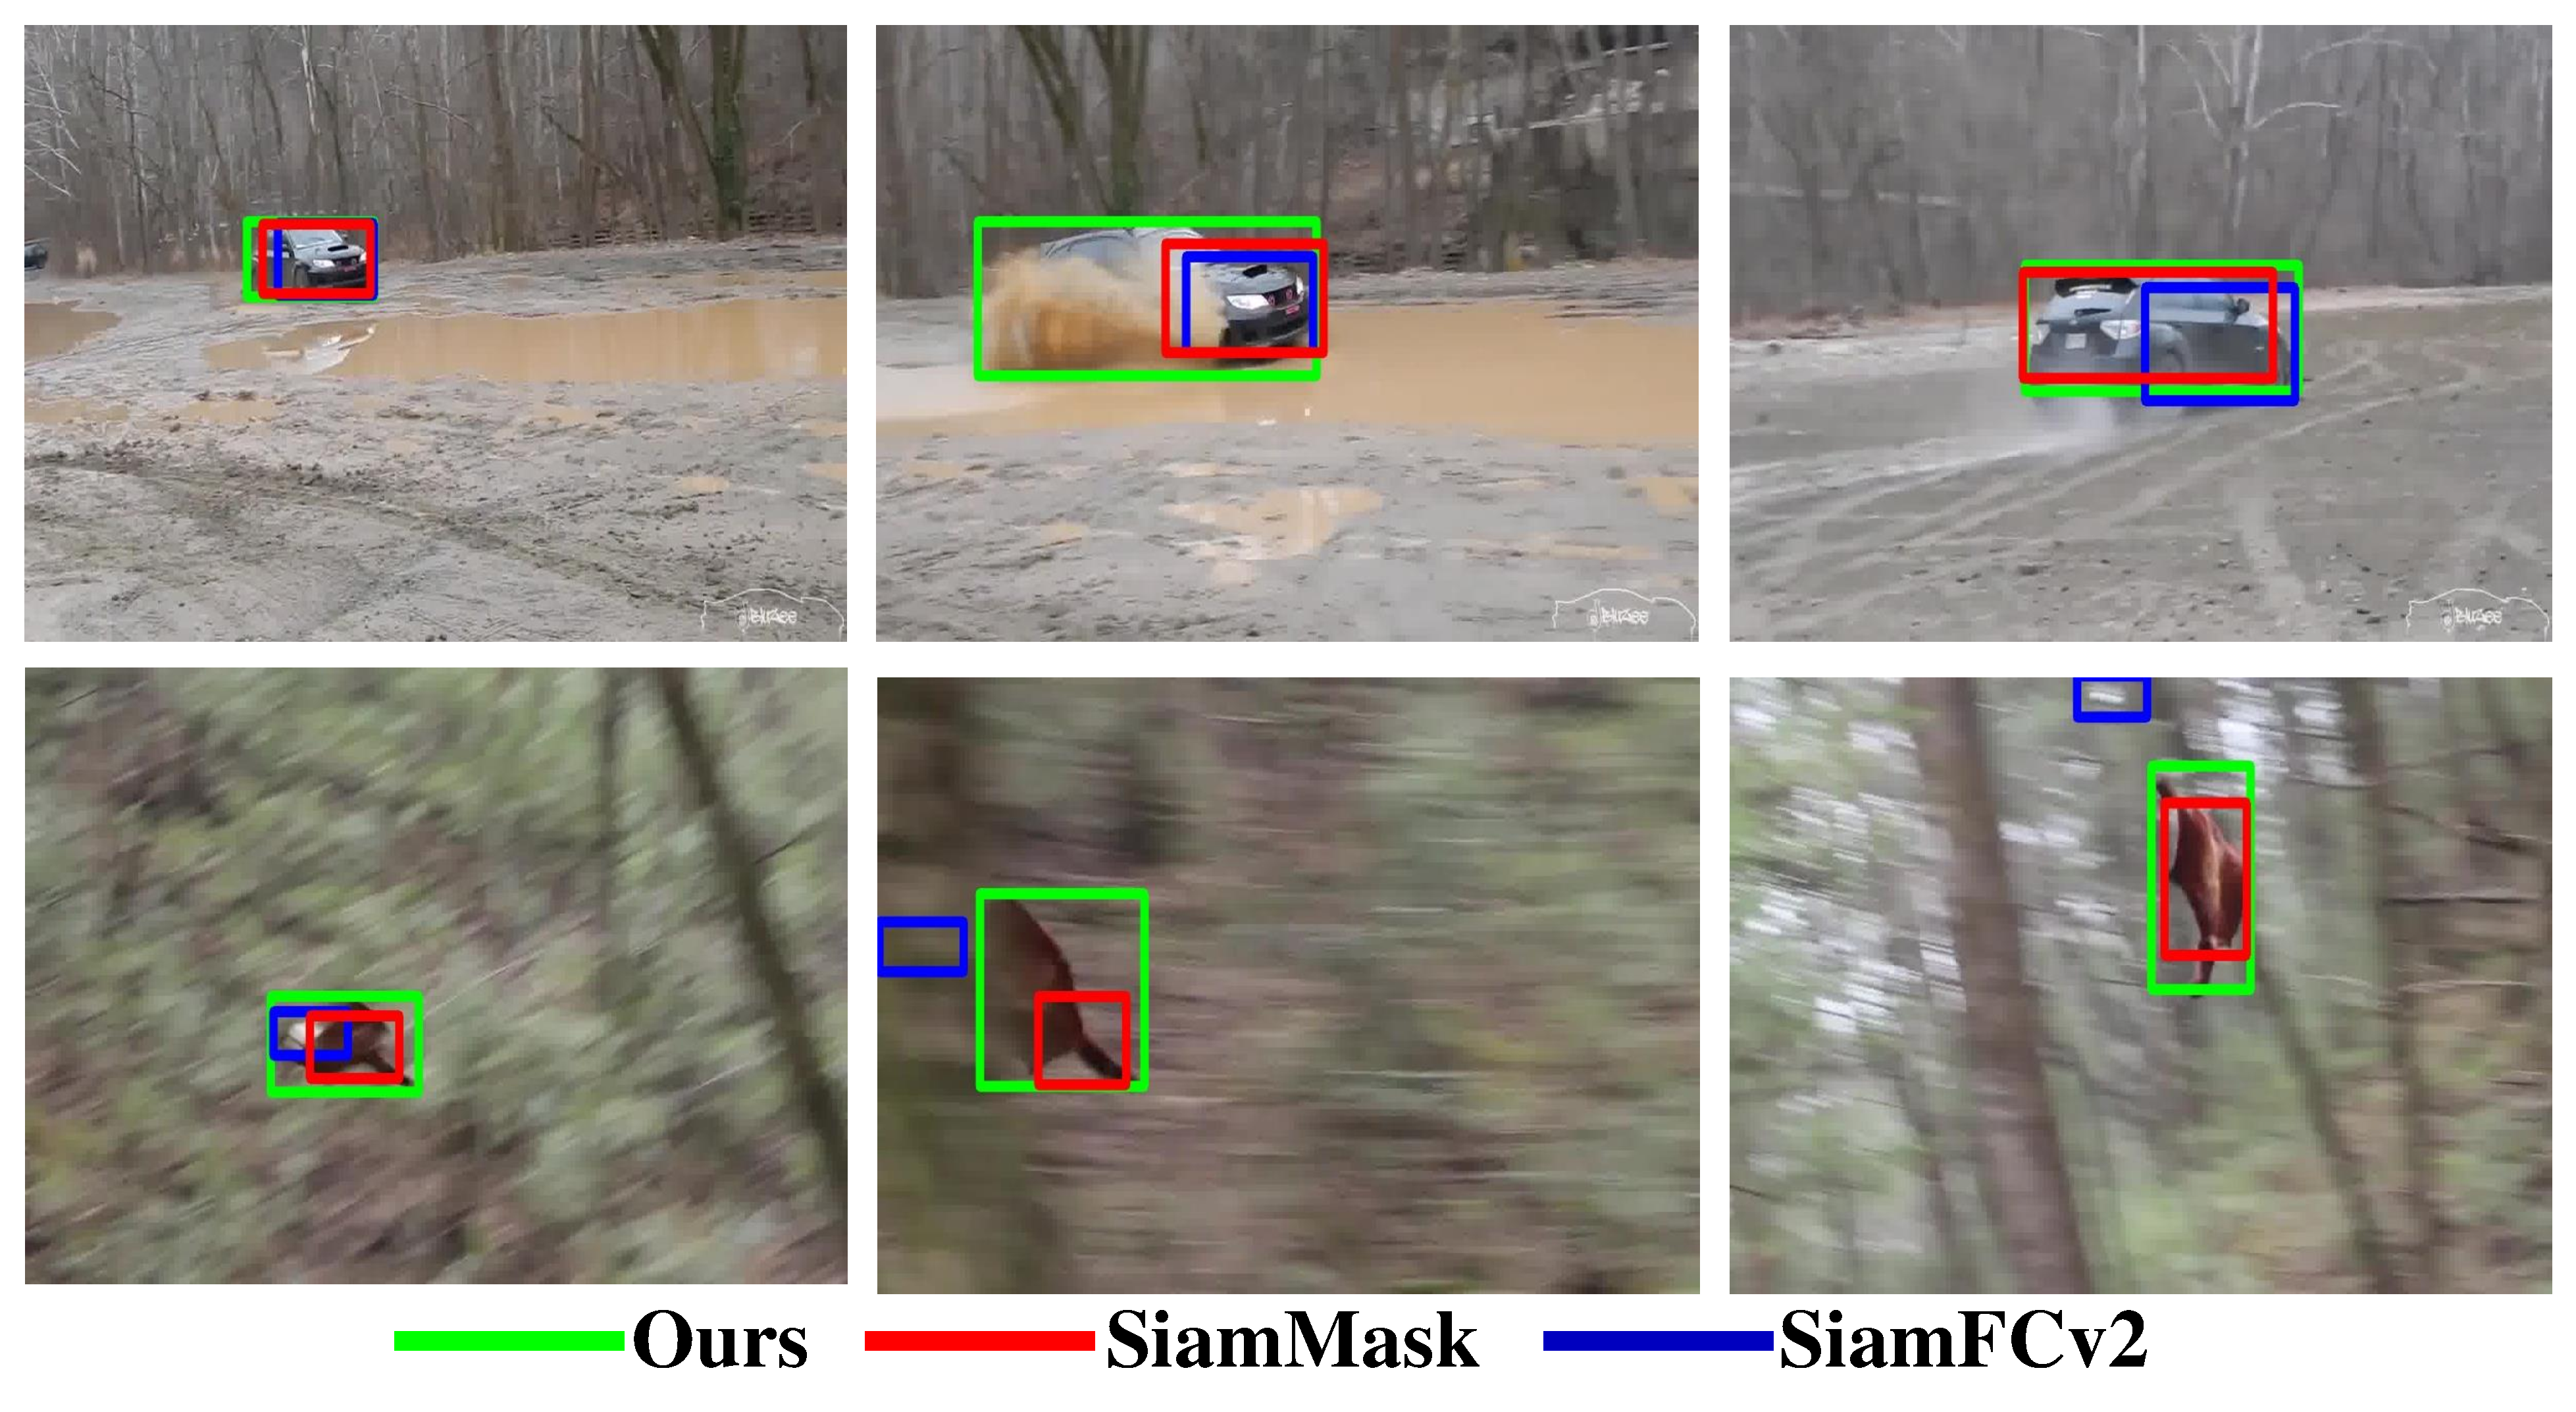
\includegraphics[width=0.48\textwidth]{Img/end/visulization.pdf}
    \caption{A comparison of our method with SiamMask and SiamFCv2. The example frames are from the GOT-10k testing set. Our approach effectively handles poor object appearance compared to existing approaches.}
    \label{fig:visulization}
\end{figure}

Actually, the video has rich information about the target and such temporal information is an important basis for video understanding and tracking.
For example, in video object detection, FGFA \cite{zhu2017flow} leverages temporal coherence on feature level. It improves the per-frame features by aggregation of nearby features along the motion paths, and thus improves the video recognition accuracy.
In video object segmentation, STCNN \cite{xu2019spatiotemporal} introduces a temporal coherence module, which focuses on capturing the dynamic appearance and motion cues to provide the guidance of object segmentation.
In discriminative correlation filter-based object tracking, FlowTrack \cite{zhu2018end} focuses on making use of the rich flow information in consecutive frames to improve the feature representation and the tracking accuracy. 
However, how to utilize the temporal information in siamese trackers has not been widely studied yet. 

\begin{figure*}[t]
    \centering
    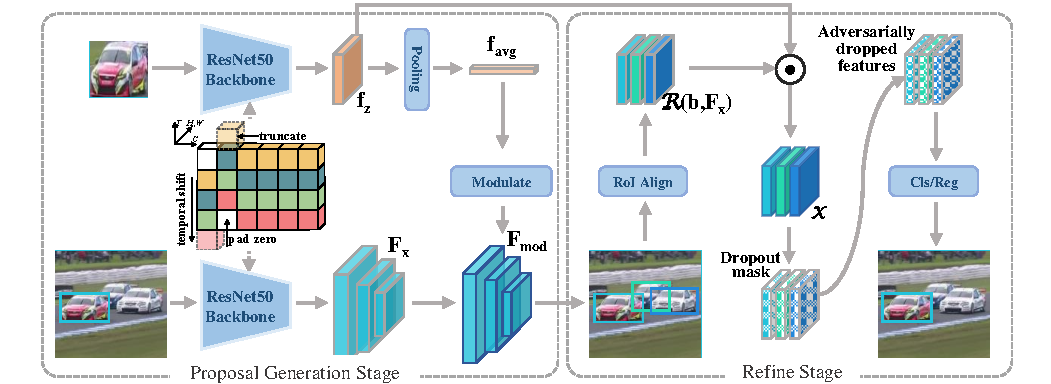
\includegraphics[width=0.9\textwidth]{Img/end/net_v3.pdf}
    \caption{
    Overview of our two-stage SiamTFA.
    %At the first stage, a siamese FPN equipped with a temporal aggregation module provides features of the template image and the search image. Then the feature modulation module is used to merge the features and generate proposals.
    %proposals of the object given in the first-frame bounding box. 
    %At the second stage, 
    The proposal generation stage aims to generate proposals that are visually similar to the given template target. The refine stage aims to select the target from candidate proposals.}
    \label{fig:SiamTFA}
\end{figure*}

% key words: temporal modeling, model the temporal information, temporal fusion, inter-frame information, improve the feature representation, temporal aggregation, poor object appearance
In this paper, we aim to take full advantage of temporal information in siamese trackers.
%(We introduce a novel siamese tracking architecture equipped with a temporal aggregation module to make full use of inter-frame information.)
%(In this work, to deal with the issues raised above, we propose a novel tracker to aggregate features of adjacent frames by ...)
%(In this paper, we develop an end-to-end temporal aggregation module in siamese architecture to utilize both the power of siamese trackers and the inter-frame information.)
We introduce a novel siamese tracking architecture equipped with a temporal aggregation module, which improves the per-frame features by aggregating features from adjacent frames.
This temporal fusion strategy enables the siamese tracker to handle poor object appearance like motion blur, occlusion, \textit{etc}.
To achieve this, we shift the channels along the temporal dimension \cite{lin2019tsm} in the backbone of the siamese network.
Note that features of the same object are usually not spatially aligned across frames due to video motion \cite{zhu2017flow}, so the temporal shift is only performed on the residual layers \cite{lin2019tsm} to preserve the spatial feature learning capability of the siamese tracker.
Different from other temporal fusion methods \cite{tao2016siamese, gladh2016deep}, the proposed method is able to be trained end-to-end on large-scale datasets.
%The proposed temporal aggregation module is trained end-to-end in the siamese network.
%(This module enables our module to be trained end-to-end on large-scale datasets.)
Additionally, our temporal fusion method is easy to implement, without changing the siamese tracking architecture or using optical flow \cite{zhu2018end}.

%improve the generalization ability on bad object.
%Our insight is that, if we only rely on the traditional training method, the bad image in the training data will be over wheeled by the easy cases. So the tracker shows bad performance when meeting with bad image during testing. To solve this problem, we take advantage of the recent progress in adversarial learning to increase the robustness of object features.
%Our method employs adversarial dropout to increase the robustness of object features. 
%注意,由于该模块在文章中占据次要位置,所以不应该写目前方法存在的缺点,而应该直接写用了这个模块后起到的作用。
%感觉概括性的优点不太好想,所以可以多些几句实现细节。这就要求我们弄懂代码原理。
To improve the robustness of target features, we further incorporate an adversarial dropout \cite{park2018adversarial} module in the siamese tracking network.
% add adversarial dropout to enforce the tracker to learn difficult cases. 
% (We further propose a adversarial training module to enforce the tracker to learn difficult cases. The motivation is that ... This is achieved by computing the adversarial masks based on diversity maximum. This simple form of feature selection improves the discrimination power of the tracker.)
%Specifically, we calculate the diversity of two dropouts, and make the loss max to learn the difficult dropout mask.
Specifically, we first predict adversarial dropout masks based on divergence maximum.
Then, we aim to minimize the divergence between the randomly dropped features and the adversarially dropped features.
%The effect of this module can be interpreted from both the dropout and from the adversarial training perspectives.
This module has both the advantages of dropout and adversarial training: the dropout makes our siamese network randomly disconnects neural units during training to prevent the co-adaptation of target features and the adversarial training enforces our tracker to learn difficult cases.

\iffalse
Our contributions are three folds:
(1) We introduce a novel siamese tracking architecture equipped with a temporal aggregation module, which improves the per-frame features by aggregating features of adjacent frames.
(2) We incorporate the adversarial dropout module in our tracker to improve the discrimination power of the siamese tracking network.
(3) Experiments on GOT-10k and UAV20L tracking datasets show that the proposed method performs favorably against existing state-of-the-art methods (Fig. \ref{fig:visulization}).
\fi
\iffalse
\begin{itemize}
    \item We introduce a novel siamese tracking architecture equipped with a temporal aggregation module, which improves the per-frame features by aggregating features of adjacent frames.
    \item We utilize the adversarial dropout module to improve the discrimination power of the siamese tracking network.
    \item Experiments on GOT-10k and UAV20L tracking datasets show that the proposed method performs favorably against existing state-of-the-art methods.
\end{itemize}
\fi

\section{The proposed Method}
\label{sec:method}
%应该提及我们的跟踪器的损失函数包括:对抗性损失,加上常规跟踪损失。
%In this section, we will introduce the proposed tracking method, SiamTFA (Fig. \ref{fig:SiamTFA}). 
%The main feature is:
%(1) A strong backbone. Use FPN and new-proposed feature modulation.
%(2) Equipped with 2 useful module: temporal aggregation module and adversarial dropout module to improve the robustness of features.
%In the following, three sub-section will be introduced: (1) Overview of tracking (2) Temporal aggregation module (3) Adversarial dropout module.
%网络结构怎么描述?可以参考ATOM。
%Our SiamTFA bases on a strong feature extractor -- FPN.
%We insert our temporal aggregation module in the backbone. Details of this module will be introduced at sec 3.2.
%Be robust to object size.
%FPN: handle different object size.
%modulator vector: handle different template object size.
%xcorr depth-wise: stage1 merge.
%element wise product: stage2 merge
% 介绍输入
%The input of the network is ... We use notations ... to denote ..., respectively. ... has a size of ...
%SiamTFA is composed of ... and ...
%Inspired by the great success of siamese trackers \cite{li2019siamrpn++, wang2019fast}, we also construct our SiamTFA based on the siamese architecture.
In this section, we will introduce the proposed siamese architecture-based tracking method, namely SiamTFA (Fig. \ref{fig:SiamTFA}), which is inspired by the great success of siamese trackers \cite{li2019siamrpn++, wang2019fast}.
Specifically, SiamTFA takes an image pair as input, comprising a template image and a search image. The template image is the image patch cropped from the initial frame according to ground truth bounding box. The search image is one whole frame in the remaining of the video. Both inputs share the same feature extractor and parameters.
Inspired by the success of the two stage detection paradigm \cite{ren2015faster}, our siamese tracker is also a two stage method. The first stage aims to generate proposals that are visually similar to the given template target. In this stage, we introduce a temporal aggregation module
%(Fig. \ref{fig:TSM}) 
to enhance the temporal information (Sec. \ref{sec:stage1}). The second stage aims to
identify the target from candidate proposals.
% select the target from candidate proposals. 
In this stage, we insert an adversarial dropout module to learn more robust features (Sec. \ref{sec:stage2}).

\subsection{Temporal aggregation module}
\label{sec:stage1}
% Note that 'stage1' and 'stage2' is a local term. You should introduce the global architecture which includes 'stage1' and 'stage2' first.
% You need to say something about ‘siamese' and the 'input'.
The proposal generation stage consists of 3 components: (1) feature extractor, (2) temporal aggregation module, and (3) feature modulation module.
% 需要综述三个模块在stage1中的作用。
The feature extractor generates the search features and the template feature for the search image and the template image, respectively. The temporal aggregation module is integrated into the feature extractor to utilize the temporal information. The feature modulation module merge the search features and the template feature to recognize the candidate targets.

\textbf{Feature extractor} To deal with the scale change of the target, we use Res50-FPN \cite{lin2017feature} as our feature extractor.
% You need to describe FPN here. What is FPN?
\textbf{F}eature \textbf{P}yramid \textbf{N}etwork (FPN) exploits the inherent multi-scale,  pyramidal hierarchy of deep convolutional networks to construct feature pyramids with marginal extra cost. 
Our siamese FPN takes a template image and a search image as input. For the search image, the FPN outputs proportionally sized feature maps at multiple levels, in a fully convolutional fashion.
%The input of the feature extractor is an image pair consists of a template image and a search image. The search image is resized to min size 800. The template is cropped according to ground truth bounding box and resized into 400*400. According to the siamese architecture, the template/search image share the same parameters. 
%For the search image, we got 5 different features and they have strides of \{4, 8, 16, 32, 64\} pixels with respect to the input image. For template branch, we use the last layer of FPN with size 7*7. 
We denote the output for the search image as $F_{x} = \{f_{x}^i\}_{i=1:5}$, and note that they have strides of \{4, 8, 16, 32, 64\} pixels with respect to the input search image.
For the template image, we use the last stage of the FPN output as the template feature with a spatial size of $7 \times 7$.
%Different from traditional trackers, our template/search features have temporal information. The reason is because we insert the temporal shift module into the backbone, which will be introduced next.

\textbf{Temporal aggregation module}
%Different from traditional trackers, we use the rich information about the same object instance by 
Most popular siamese trackers \cite{li2019siamrpn++, wang2019fast} use the still image to make prediction. % However, tracking on single frame generates unstable results and fails when appearance is pool \cite{zhu2017flow}. 
This limits the ability of these siamese trackers.
On one hand, tracking on single frame generates unstable results and fails when appearance is poor (Fig. \ref{fig:visulization}); on the other hand, 
temporal adjacent frames can provide more information about the target.
%the video has rich information about the target. 
So we aim to improve the per-frame features by aggregating features of adjacent frames.
Specifically, we insert a temporal aggregation module into the last stage of the feature extractor. 
% We have to cite TSM, because we use this idea.
To model temporal information, the images in one batch are several adjacent frames in the same video and are sorted by time, so we can regard the batch dimension as the time dimension. Assume the feature map at the last stage of the feature extractor is $f \in \mathbb R ^ {T \times C \times H \times W}$.
For each time $t \leq T$, we first split feature $f^t \in \mathbb R ^ {C \times H \times W}$ into 3 parts along the channel dimension: $f_{1:K}^t \in \mathbb R ^ {K \times H \times W}$, $f_{(K+1):2K}^t \in \mathbb R ^ {K \times H \times W}$, and $f_{(2K+1):C}^t \in \mathbb R ^ {(C-2K) \times H \times W}$.
Then we shifts the channels along the temporal dimension following \cite{lin2019tsm}:
% Then The aggregated function at time $t$ is:
\begin{equation}
    f_{agg}^t = \mathcal{C}(f_{{1:K}}^{t-1}, f_{(K+1):2K}^{t+1}, f_{(2K+1):C}^{t}),
\end{equation}
where $\mathcal{C}(\cdot)$ is the concatenation operation. According to \cite{lin2019tsm}, the shift operation is only performed at the residual layer to preserve the spatial feature learning capability of the siamese tracker.
Note that the aggregated feature $f_{agg}^t$ has the same shape with $f^t$, so we can insert this module into the backbone directly, without the need to change other part of the network.
What's more, this operation only needs to do data movement, so it is computationally free and can be trained end-to-end.
% Say the effect of this module.
%After performing such channel fusion, rich target information in adjacent frames can be aggregated into the current frame. For example, if the current frame is blurred, target information that is not blurred in adjacent frames can be used.

\iffalse
\begin{figure}[t]
    \centering
    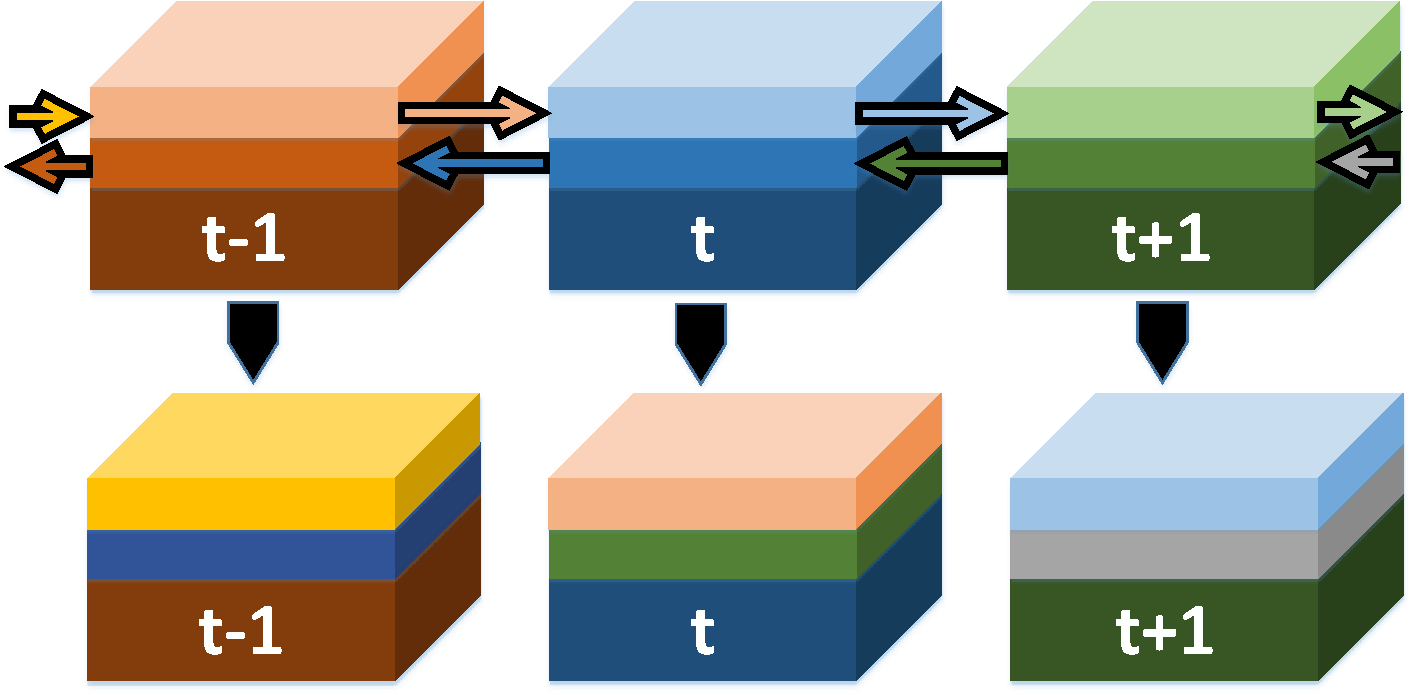
\includegraphics[width=0.4\textwidth]{images/TSM_v1.pdf}
    \caption{Temporal aggregation module.}
    \label{fig:TSM}
\end{figure}
\fi

\textbf{Feature modulation module} After getting the template feature $f_{z}$ and the search feature pyramid $F_{x} = \{f_{x}^i\}_{i=1:5}$, they are modulated to generate target-specific features.
Specifically, The modulation vector $f_{avg}$ is generated from $f_{z}$ using global average pooling, which carries the target-specific appearance information. 
%The search feature pyramid is $F = \{f_1, f_2, f_3\}$. 
%For $f_{x}^{i} \in F_{x}$, t
The modulated feature pyramid $F_{mod} = \{f_{mod}^i\}_{i=1:5}$ is generated as follows:
\begin{equation}
    f_{mod}^i = \mathcal{M}(f_{avg}, f^i_x),
\end{equation}
where $\mathcal M(\cdot)$ is the depth-wise correlation \cite{li2019siamrpn++}.
%So we get the modulated feature pyramid $F_{mod} = \{f_{mod}^i\}_{i=1:5}$. 
%Then we predict proposals on $F_{mod}$.
Each modulated feature map is fed into two sibling fully-connected layers---a box-regression layer with channel dimension 4$k$, and a box classification layer with channel dimension 2$k$, where $k$ is the number of maximum possible proposals for each location.
% anchor 这个概念是必备的,所以是得讲一下。
The object/background criterion and bounding box regression are defined with respect to a set of anchors.
Following \cite{lin2017feature}, we assign anchors with the same scale to each of the different pyramid levels. For detail information of the anchor setting, please refer to \cite{lin2017feature}.
% For every modulated layer, we attach a classification layer and a regression layer to make predict.
\iffalse
The loss function of stage 1 is:
\begin{equation}
    \mathcal{L}_1 = 
\end{equation}
\fi
% you need to say how we get the candidates. Faster R-CNN already says it.
%The generated proposes with top-K classification scores is send to stage2.
We use the top-$N$ ranked proposal regions for the refine stage.

\subsection{Adversarial dropout module}
%stage 1 的网络结构已经交代清楚了,就是一个FPN。和调制,和分类/回归层。那么stage的网络结构也应该交代清楚:roi align + 特征融合 + 对抗 + 分类/回归层。
\label{sec:stage2}
% 首先你要讲一下stage2在全局中的作用。
The refine stage aims to select the target from candidate proposals.
% 或许该讲一下stage2的输入包括:真实目标特征+候选区域。
% The input of stage 2 consists of: (1) The target feature is $f_{z} \in \mathbb R ^{256 \times 7 \times 7}$. (2) The candidate boxes generated from stage 1.
% Stage 2 compose of a feature merge module, a adversarial dropout module, a classifier layer $h^{cls}$ and a regression layer $h^{reg}$. 
Features of these candidate proposals are cropped from the search feature pyramid $F_{x}$ using RoIAlign \cite{he2017mask}, and then fused with the target feature $f_{z}$:
\begin{equation}
    \mathcal{X} = \mathcal{R}(b, F_{x}) \odot f_{z},
\end{equation}
where $\mathcal{R}$ represents the RoIAlign, $\odot$ represents the element-wise multiplication, $b$ represents an RoI in candidate proposals and $\mathcal{X}$ represents the fused feature of $b$.
%where $x' \in \mathbb R ^{256 \times 7 \times 7}$.
%$x' \in \mathbb R ^{256 \times 7 \times 7}$ is the feature of an RoI cropped from unmodulated feature pyramid using RoIAlign \cite{he2017mask}.
%The merged feature of a candidate target is:$x = x' \odot x_0$, where $\odot$ represents the element-wise multiplication. $x$ is the merged feature of that RoI.
% Maybe you need to say why you do the merge again.
% The modulation in stage 1 and the feature merge in stage 2 play different part in the tracking process. The modulation aims to detect the similar appearance in the whole image. The

\textbf{Adversarial dropout} After the feature fusion, we use adversarial dropout \cite{park2018adversarial, lee2019drop} to increase the discriminative ability of $\mathcal{X}$.
% 简短的描述你是怎么做的。这是很重要的,让读者先对你的东西有个大概的了解,才能进一步了解细节。
We first predict the adversarial dropout mask based on divergence maximum. The mask is applied to $\mathcal{X}$ to get the adversarially dropped features.
Then, we aim to minimize the divergence between the randomly dropped features and the adversarially dropped features.
%Specifically, we donate the random mask as $m^s$, the adversarial mask as $m^{adv}$.
Specifically, let $h^{cls}$ and $h^{reg}$ denote the classification layer and the regression layer in stage 2, respectively.
The adversarial dropout mask is calculated as follows according to \cite{lee2019drop}:
\begin{equation}
\begin{split}
    & \mathbf{m}^{adv} = \mathop{\arg\max}\limits_{\mathbf{m}}D[h^{cls}(\mathcal{X} \odot \mathbf{m}^s), h^{cls}(\mathcal{X} \odot \mathbf{m})] \\
    & where~||\mathbf{m}^s - \mathbf{m}|| \leq \delta_e L,
\end{split}
\end{equation}
where $L$ represents the dimension of $\mathbf{m} \in \mathbb R^L$,
$\mathbf{m}^s$ represents the random mask and $\mathbf{m}^{adv}$ represents the adversarial mask.
$\delta_{e}$ is a hyper parameter to control the perturbation magnitude with respect to $\mathbf{m}^{s}$ \cite{lee2019drop}.
%and $\delta_{e}$ is a hyper parameter to control the perturbation magnitude with respect to $m^{s}$ \cite{lee2019drop}
$D[p, p']  \geq 0$ measures the divergence between two distributions $p$ and $p'$.

To calculate $\mathbf{m}^{adv}$, \cite{park2018adversarial} optimizes a 0/1 knapsack problem with appropriate relaxations in the process. Please refer to \cite{park2018adversarial} for detail information.
%Then, we use the mask to dropout the feature, then send it to the classifier.
%We also send the clean feature to the classifier, and wish the loss minimum:
After generating $\mathbf{m}^{adv}$, we then aim to minimize the divergence between two predicted distribution regarding to $\mathcal{X}$: one with a random dropout mask $\mathbf{m}^{s}$ and another with an adversarial dropout mask $\mathbf{m}^{adv}$ \cite{lee2019drop}.
\begin{equation}
    \mathcal{L}_{adv} = \mathbb E[D_{KL}[h^{cls}(\mathcal{X} \odot\mathbf{m}^{s})||h^{cls}(\mathcal{X} \odot\mathbf{m}^{adv}))]],
\end{equation}
where $D_{KL}$ is the Kullback-Leibler divergence.

Finally, for each RoI, the classification layer produces softmax probability estimates over two classes (foreground or background) and the regression layer outputs four real-valued numbers for the foreground class. These four values encode the refined bounding-box position for the RoI.
The loss of SiamTFA is:
%The RoI Aligned features are fed into the global average pooling layer followed by two sibling output layers: one that produces softmax probability estimates over two classes (foreground or background) and another layer that outputs four real-valued numbers for the foreground class. These four values encode the refined bounding-box position for the RoI.
%We get the final tracking result as follows: The classification layer $h^{cls}$ predicts a score for a RoI, the regression layer $h^{reg}$ has shape * and predicts a 4-d vector for it.
%The RoI with the top score is the final box.
\begin{equation}
\mathcal{L} = \mathcal{L}_{cls}^{stage1} + \mathcal{L}_{cls}^{stage2} + \mathcal{L}_{reg}^{stage1}+\mathcal{L}_{reg}^{stage2} +  \lambda \mathcal{L}_{adv},
\end{equation}
where $\lambda$ is a hyper-parameter to balance the adversarial loss and the classification/regression loss. $\mathcal{L}_{cls}^{\cdot}$ is the cross entropy loss and $\mathcal{L}_{reg}^{\cdot}$ is the standard smooth $L1$ loss for regression. During testing, the RoI with the top classification score is selected as the predicted target.


\iffalse
{classification/regression} The structure of $f^{cls}$ is ... The structure of $f^{reg}$ is ...
Suppose $B^*_t$ is the target bounding box at frame $t$, which is estimated through:
\begin{equation}
B^*_t = h^{reg}(\mathop{\arg\max}\limits_{x \in \mathcal{X}}h^{cls}(x)), 
\end{equation}
where $\mathcal{B}_t^1$ is a set of proposals generated from stage 1.
\fi

\section{Experiments}
In this section, we first present the implementation details.
Then we evaluate out method on GOT-10K \cite{Huang_2019} testing set and the UAV20L \cite{mueller2016benchmark} dataset.
\subsection{ Implementation details}
The proposed network is trained on the training set of GOT-10k \cite{Huang_2019} and the backbone is pretrained on ImageNet.
We apply stochastic gradient descent with momentum of 0.9 and set the weight decay to 0.0005.
The learning rate is decreased from $10^{-2}$ to $10^{-4}$.
The batch size is set to 2 and the network is trained for 90000 iterations.
Our tracker is implemented in Python, using PyTorch.
%First stage, we select 4000 proposals to send to stage2, the positive/negative rate is 1:3.
%To shift channels $K=2$.
%Because of the memory limit, the batch size is 2.
%To calculate the loss, $\lambda = 1$.
%For both training and testing, the size of a template image is 
% 其实有些对不上。按论文上讲,第一阶段是找到若干候选框。第二阶段是得到唯一结果。实际上是,第一阶段得到若干候选框,第二阶段进一步筛选得到约10个候选框(这才是真正的相似目标),然后按IoU和得分来选择最终结果。
% For test, we select top 100 proposals to send to stage2. The we use NMS to select top 10 object. 
\subsection{Evaluation on GOT-10k dataset}

\iffalse
\begin{figure}[t]
    \centering
    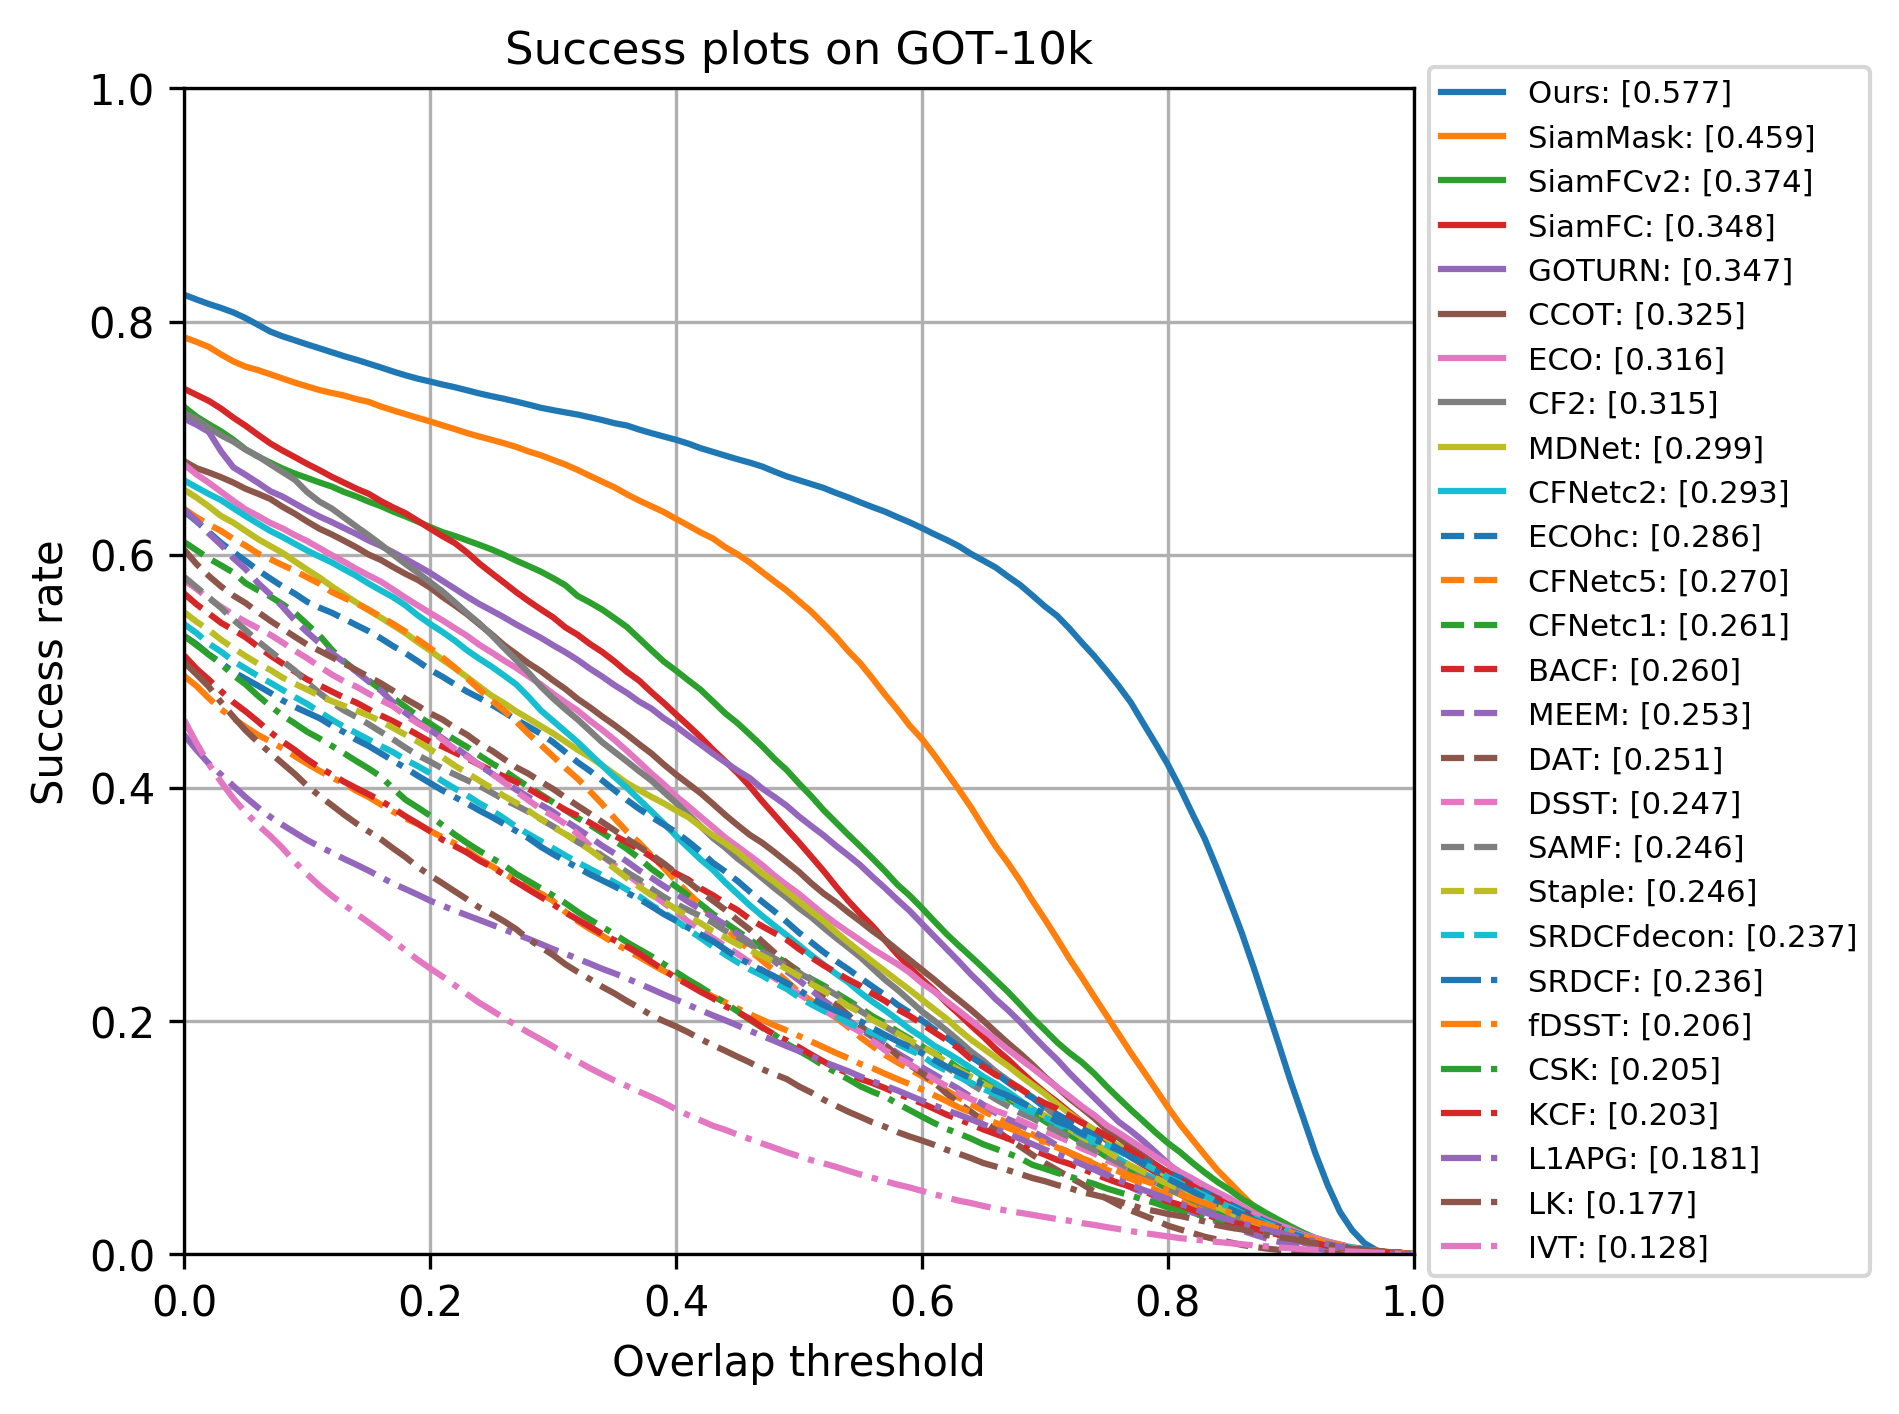
\includegraphics[width=0.45\textwidth]{images/success_plot.png}
    \caption{Overall performance on GOT-10k, ranked by their average overlap (AO) scores.}
    \label{fig:got10k}
\end{figure}
\fi
\begin{table}
\centering
\caption{Performance of our algorithm with different components on GOT-10k test set.}
\begin{tabular}{c c c c c}
\bottomrule
\begin{tabular}[x]{@{}c@{}}Temporal\\aggregation\end{tabular} & \begin{tabular}[x]{@{}c@{}}Adversarial\\dropout\end{tabular} & $AO$ & $SR_{0.50}$ & $SR_{0.75}$ \\ 
\hline
          &           & 0.542 & 0.607 & 0.456 \\
\checkmark&           & 0.561 & 0.645 & 0.480 \\
\checkmark&\checkmark & 0.577 & 0.662 & 0.509 \\
\bottomrule
\label{tabel:ablation}
\end{tabular}
\end{table}
\begin{table}
\centering
\caption{Comparing the results of our approach against other approaches over the GOT-10k test set.}
\begin{tabular}{l l l l}
\bottomrule
Method   &  $AO$   &  $SR_{0.50}$ & $SR_{0.75}$  \\
\hline
Ours &  $\textbf{0.577}^\textbf{1}$ & $\textbf{0.662}^\textbf{1}$  & $\textbf{0.509}^\textbf{1}$  \\
SiamMask &  0.459&  0.560 &0.205 \\
SiamFCv2 &  0.374&  0.404 &0.144 \\
SiamFC   &  0.348&  0.353 &0.098 \\
GOTURN	 &  0.347&  0.375 &0.124 \\
CCOT	 &  0.325&  0.328 &0.107 \\
ECO	     &  0.316&  0.309 &0.111 \\
CF2	     &  0.315&  0.297 &0.088 \\
MDNet	 &  0.299&  0.303 &0.099 \\
%CFNetc2	 &  0.293&  0.265 &0.087 \\
%ECOhc	 &  0.286&  0.276 &0.096 \\
\bottomrule
\end{tabular}
\label{table:got}
\end{table}
In this subsection, we evaluate our method on GOT-10k \cite{Huang_2019} dataset.
% Say something about this dataset.
GOT-10k is a recent large-scale high-diversity dataset consisting of over 10,000 video sequences with targets annotated by axis-aligned bounding boxes. 
%Note that the classes between training and test sets are zero-overlapped. 
%This one-shot protocol avoids the evaluation bias towards familiar objects. 
The GOT-10k testing set includes 180 sequences with 84 different object classes and 32 motion patterns. As performance measure, we use the average overlap (AO) scores and success rate (SR) as proposed in \cite{Huang_2019}. The AO denotes the average of overlaps between all groundtruth and estimated bounding boxes, while the SR measures the percentage of successfully tracked frames where the overlaps exceed 0.5/0.75.

\textbf{Ablation Studies}
From Table \ref{tabel:ablation} (the $1^{st}$ and $2^{nd}$ row), we see that the AO performance increases by 1.9\% by adding the temporal aggregation module.
This is because the temporal aggregation module improves the per-frame features by aggregating temporal information from adjacent frames.
%The RPN stage rapidly filters out most background samples, and the RoI head adopts a fixed foreground-to-background ratio to maintain a manageable balance between foreground and background.
From Table \ref{tabel:ablation} (the $2^{nd}$ and $3^{rd}$ row), we see that with the adversarial dropout module, the AO increases by 1.6\%.
%This is because the proposed motion model can effectively predict the position distribution of the target, effectively avoiding the adverse effects of distractors. 
This is because the adversarial dropout module improves the discrimination power of our siamese tracking network.

\textbf{Overall Performance}
We compare our proposed method with 8 trackers, including state-of-the-arts.
The performances of the evaluated trackers is shown in Table \ref{table:got}.
Compared to other listed approaches, our approach achieves a superior AO of 0.577.
%ECO \cite{danelljan2017eco} is a state-of-the-art DCF-based tracker, which introduces a factorized convolution operator that dramatically reduces the number of parameters in the DCF model. In contrast, our tracker is based on the powerful siamese architecture. As a result, our tracker significantly outperforms ECO with a gain of 26.1\% in terms of AO score, which suggests the effectiveness of the siamese architecture for the object tracking task.
%SiamMask \cite{wang2019fast} is a recently proposed siamese tracker. It simultaneously trains a siamese network on three tasks, each corresponding to a different strategy to establish correspondences between the target object and candidate regions in the new frames.
% However, it is based on the local search mechanism: searching the target within a small neighborhood centered on the target position of the previous frame. In the contrast, our SiamTFA use the the global search mechanism. It is always able to perceive the target over the entire image. As a result, our tracker outperforms SiamMask by relative * in terms of AO, which highlights ...
Compared with SiamMask, our tracker aims to make full use of the temporal information. As a result, our tracker outperforms SiamMask by 11.8\% in terms of AO, which highlights the importance of the proposed temporal aggregation module.

\begin{figure}[t]
\begin{minipage}[b]{.48\linewidth}
  \centering
  \centerline{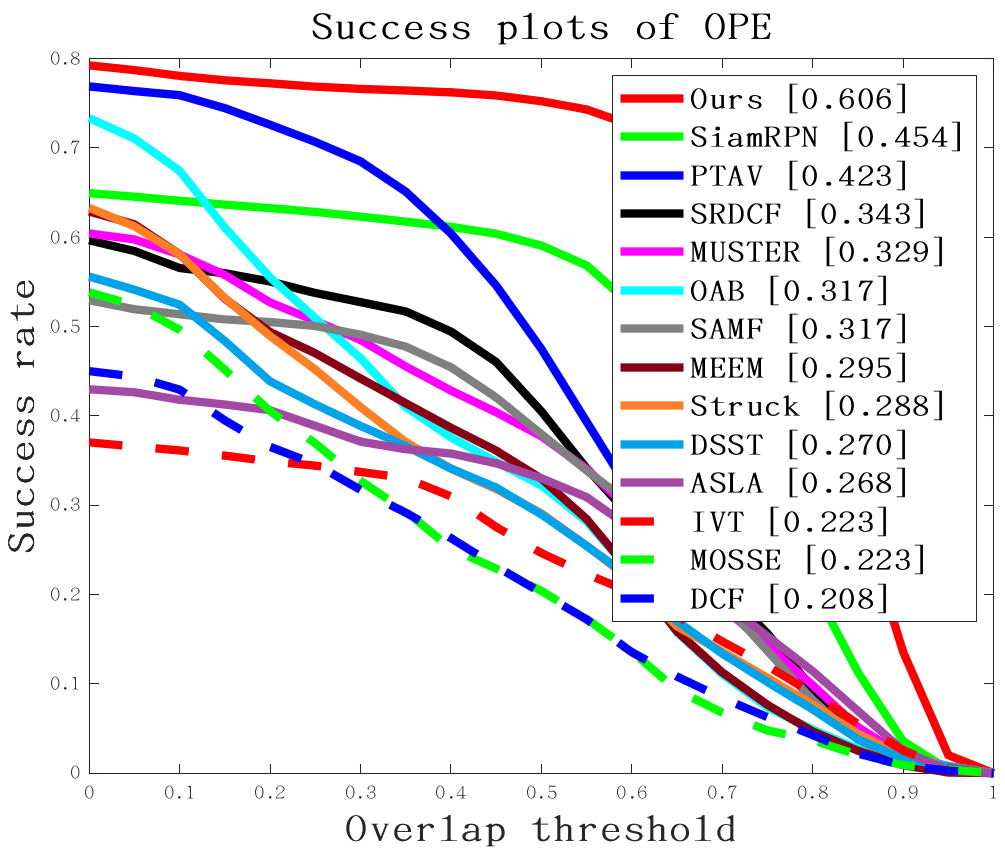
\includegraphics[width=5.0cm]{Img/end/quality_plot_overlap_OPE_AUC.png}}
\end{minipage}
\hfill
\begin{minipage}[b]{0.48\linewidth}
  \centering
  \centerline{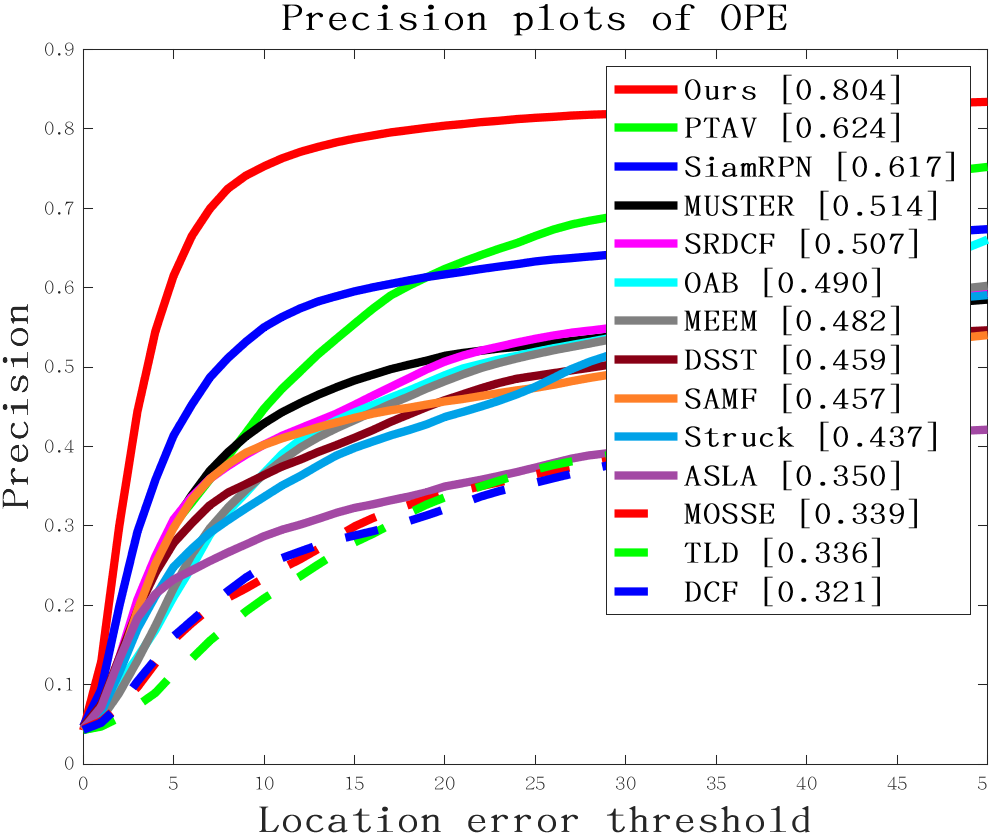
\includegraphics[width=5.0cm]{Img/end/quality_plot_error_OPE_threshold.png}}
\end{minipage}
%
\caption{Success and precision plots on UAV20L dataset.}
\label{fig:uav20l}
%
\end{figure}
\subsection{Evaluation on UAV20L dataset}
In this subsection, we evaluate our tracker on the UAV20L \cite{mueller2016benchmark} long term tracking dataset.
% say something about this dataset: length, 20段
It contains 20 HD video sequences captured from a low-altitude aerial perspective with average sequence length of 2934 frames.
% It has mean frames of 2934 and max frames of 5527.
% say something about the measures. 
In this experiment, all trackers are compared using two measures: precision and success. Precision is measured as the distance between the centers of the predicted bounding box and the corresponding ground truth bounding box. Success is measured as the intersection over union of pixels in predicted bounding box and those in ground truth bounding box.
% say something about the accuracy.
In Fig. \ref{fig:uav20l}, we can find that the proposed algorithm achieves better tracking performance compared with some representative trackers.
In the success plot, our tracker obtains an AUC score of 0.606.
% PTAV is ... Compared with it, our is higher. This demonstrates the effectiveness of our designed architecture.
In the precision plot, the proposed algorithm obtains a score of 0.804.
% MUSTER is ... Compared with it, our is higher.
It shows that our tracker surpass other state-of-the-art algorithms, such as SiamRPN \cite{li2018high} and PTAV \cite{fan2017parallel}. This demonstrates the effectiveness of our tracker in long-term tracking scenario. 
%designed architecture.
%It shows that our tracker surpass another siamese tracker -- SiamRPN. This demonstrates the effectiveness of our designed architecture. Moreover, compared with other state-of-the-art algorithms, such as PTAV \cite{} and MUSTER \cite{}, our trackers are still superior in terms of precision.
\section{Conclusion}
%一句话指出我们提出了什么。
In this paper, we introduce a novel siamese architecture for visual object tracking.
Specifically, our proposed algorithm contains two main modules, \textit{i.e.} temporal aggregation module and adversarial dropout module. The temporal aggregation module improves  the per-frame features by aggregating features of adjacent frames. The adversarial dropout module improves the discrimination power of the siamese tracking network.
%say something about the experiment.
Extensive experimental results show that the proposed algorithm performs favorably against the state-of-the-art algorithms.